\documentclass{article}

\usepackage{mathrsfs,amsmath}
\usepackage{xcolor}
\usepackage{titlesec}
\usepackage{listings}
\usepackage{syntax}
\usepackage{pythonhighlighting}
\usepackage{graphicx}

\graphicspath{ {./assets/} }

\usepackage[margin=1.4in]{geometry}

\title{Handout \#2 | CS 471} 
\author{Jared Dyreson\\ 
        California State University, Fullerton}

\usepackage [english]{babel}
\usepackage [autostyle, english = american]{csquotes}
\MakeOuterQuote{"}

\titlespacing*{\section}
{0pt}{5.5ex plus 1ex minus .2ex}{4.3ex plus .2ex}
\titlespacing*{\subsection}
{0pt}{5.5ex plus 1ex minus .2ex}{4.3ex plus .2ex}

\usepackage{hyperref}
\hypersetup{
    colorlinks,
    citecolor=black,
    filecolor=black,
    linkcolor=black,
    urlcolor=black
}

\begin{document}

\maketitle
\tableofcontents

\newpage

\section{Questions}

\textbf{Note: } The Quizlet for this class can be found \href{https://quizlet.com/480232264/471-1-6-flash-cards/}{\underline{here}} and can be referenced instead of this and subsequent documents.

\begin{enumerate}

\item How does the digital subscriber line (DSL) allow telephony and Internet to co-exist on the same link?
\begin{itemize}
\item Telephony and Internet are transmitted on different frequencies thanks to the DSL modem to the DSL access multiplexer. Those different frequencies are parsed and sent to their respective destinations.
\end{itemize}
\begin{figure}[!h]
\centering
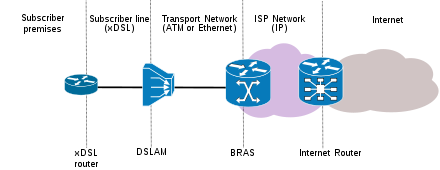
\includegraphics[width=10cm]{DSLAM_Diagram}
\caption{DSLAM Diagram}
\end{figure}

\item What is the function of the DSL access multiplexer?
\begin{itemize}
\item Connects multiple customer digital subscriber line interfaces to a high-speed digital communications channel using multiplexing techniques
\end{itemize}

\item What is the main limitation to DSL?
\begin{itemize}
\item Proximity to the DSL provider. Farther away means a weaker connection.
\end{itemize}

\item Briefly  explain  the structure  and function  of  the  hybrid  fiber  coax (HFC) approach to  connecting residences to  the  Internet. How does it differ from DSL? What are the advantages? Are there security concerns?
\begin{itemize}
\item HFC: combines optical fiber and coaxial cable. Optical uses light and coaxial employs electricity.
\item A network of cables and fiber attaches homes to the ISP router, rather than having a direct communication the central office (DSL protocol). Here, homes share access network to the cable head end.
\item Advantages: faster; 40 up and 30 down
\end{itemize}

\item What is the difference between guided and unguided media?
\begin{itemize}
\item Guided: Signal propagates in a sold media, such as wire or fiber.
\item Unguided: Signal propagates freely, such as radio waves.
\end{itemize}

\item Host A and host B are connected by two intervening routers. All intervening links have speed of 10 bps.  Suppose A wants to send a 10,000 bit packet to B. How log will it take with and without store-forward approaches?
\begin{itemize}
\item Without (unrealistic): $\frac{10000}{10} \implies 1000$ seconds.
\item With (realistic): there are three different endpoints that must be satiated. Therefore the total time is $3 \times 1000 = 3000$ seconds.
\end{itemize}

\item Why is the store-and-forward approach necessary?
\begin{itemize}
\item It ensures that the data sent by the initiator will eventually reach it's destination.
\end{itemize}

\item When can packets experience queueing delays or be lost entirely?
\begin{itemize}
\item If packets are sent faster than they can be processed (delay)
\item Packet queue is full when received (completely lost)
\end{itemize}

\item Assume that 25 users are fairly sharing a 100 bps link. How long will it take one user to transmit a 20,000 bit file?:
\begin{itemize}
\item Each user has a designated 4 BPS to themselves and using that we can calculate the time taken: $\frac{20,000 \text{ bits}}{4 \text{ bits per second}} \implies 5,000 \text{ seconds }$
\end{itemize}

\item Assuming a 1,000,000 BPS link and users who transmit at a rate of 56,000 BPS each, how many users can we support using circuit switching? Packet switching?
\begin{itemize}
\item Packet switching: $\frac{1,000,000}{56,000} \sim 17 \text{ users}$
\item Circuit switching: 1 user (direct connection, needs more resources)
\end{itemize}

\end{enumerate}

\end{document}

